\scanpage{53}
\margin{\unsure{52|25}}
\begin{flushright}4\end{flushright}

Suppose always that $\mathcal E$ is homologically connected and for the moment that the first Betti number of $\mathcal E$ is zero.

\uline{Step 1}: Construct $\Lambda(x_1,\ldots,x_n)\xrightarrow{\rho_1}\mathcal E$ where $x_1,\ldots,x_n$ are in dimension 2 and $\rho_1x_1,\ldots,\rho_1x_n$ generate $H^2\mathcal E$.
Define $d$ in $\Lambda(x_1,\ldots,x_n)$ by $dx_i=0$, $i=1,\ldots,n$.
Note that $\rho_1$ is an isomorphism on cohomology in dimension 2 and injective in dimension 3.

\uline{Step 2}: Adjoin three-dimensional variables to $\Lambda(x_1,\ldots,x_n)$ to make $\rho_1$ surjective on cohomology in dimension 3 and injective on cohomology in dimension 4.

More explicitly, we form
\[
\Lambda(x_i;y_j),\ \rho_2,\ \text{and }d.
\]
$d$ is defined by
\[
\begin{aligned}
dy_1&=0,\ldots,dy_\ell=0\\
dy_{\ell+k}&=\sum a^k_{ij}x_i\wedge x_j
\qquad k=1,\ldots,m
\end{aligned}
\]
\figure{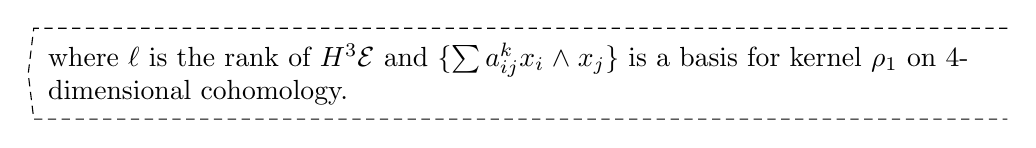
\begin{tikzpicture}
\node[anchor=north west,text width=12cm,inner sep=5pt] (p) at (0,0)
{where $\ell$ is the rank of $H^3\mathcal E$ and
$\{\sum a^k_{ij}x_i\wedge x_j\}$ is a basis for kernel $\rho_1$ on 4-dimensional cohomology.};
\draw[densely dashed] (p.north east)--(p.north west)--([xshift=-2pt]p.west)--(p.south west)--(p.south east);
\end{tikzpicture}}

$\rho_2$ is defined by choosing $\rho_2y_1,\ldots,\rho_2y_\ell$ to generate $H^3\mathcal E$ and $\rho_2(y_{\ell+k})$, $k=1,\ldots,m$, to satisfy
\[
d(\rho_2(y_{\ell+k}))=\sum_{i,j}a^k_{ij}\rho_1(x_i)\wedge\rho_1(x_j).
\]
(Now $\rho_2$ is an isomorphism on $H^3$ and injective on $H^4$.

At this point one can show by a standard Postnikov argument how this construction relates to the homotopy theory of a simply connected space $X$. If $\mathcal E$ is the de Rham
